\documentclass[dvipdfmx,tikz]{standalone}
\usepackage{tikz,bm}
\begin{document}
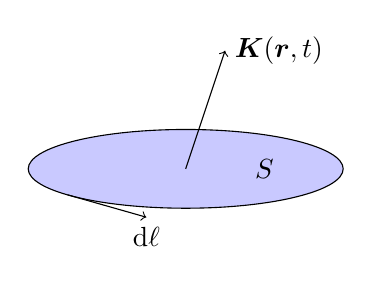
\begin{tikzpicture}
%\draw [help lines] (-2,-1) grid (2,2);
    \draw [fill = blue!30!white!70!]circle [x radius = 2, y radius = 0.5];
    \node at (1,0) {$S$};
    %\coordinate (s) at (-1.5,-0.28347335475692042041088740217563504561181348390169109075);
    \coordinate (s) at (-1.5,-0.33);
    \coordinate (g) at (-0.5,-0.61419226863999424422358937138054259882559588178699736329);
    \draw[->] (s) -- (g) node[anchor = north] {$\mathrm{d}\ell$};
    \draw[->] (0,0) -- (0.5,1.5) node[anchor = west] {$\bm{K}(\bm{r},t)$};
\end{tikzpicture}
\end{document}